\chapter{Fundamentação Teórica}
\label{cap:fundamentacao-teorica}

Este capítulo apresenta a base conceitual sobre a qual todo o restante do trabalho está construído. A \autoref{sec:rede-eletrica} define o modelo $\pi$ de rede e fixa a notação utilizada. A \autoref{sec:fp-ac} introduz o problema de Fluxo de Potência (FP) AC em coordenadas polares. A \autoref{sec:fpo-ac} estende o FP ao Fluxo de Potência Ótimo (FPO) e discute brevemente as principais relaxações disponíveis na literatura. Por fim, a \autoref{sec:acoes-controle} revisa as ações de controle do programa ANAREDE que motivam a construção das formulações \textit{hand-built} apresentadas no \autoref{chap:metodologia}.

\section{Modelagem da rede elétrica}
\label{sec:rede-eletrica}

A rede elétrica é representada por um grafo $\mathcal{G} = (\mathcal{N}, \mathcal{B})$, em que o conjunto de nós $\mathcal{N}$ corresponde às barras do sistema e o conjunto de arestas $\mathcal{B}$ aos ramos AC, abrangendo tanto linhas de transmissão quanto transformadores em fase. Adicionalmente, $\mathcal{B}_{dc}$ representa elos HVDC, $\mathcal{G}$ o conjunto de geradores, $\mathcal{L}$ o conjunto de cargas e $\mathcal{S}$ o conjunto de bancos \textit{shunt}, cada elemento associado a uma barra de $\mathcal{N}$.

Cada ramo $(i,j) \in \mathcal{B}$ é descrito pelo modelo $\pi$ clássico (\autoref{fig:modelo-pi}), com admitância série $y_{ij} = g_{ij} + j b_{ij}$, susceptâncias \textit{shunt} de extremidade $b^{fr}_{ij}$ e $b^{to}_{ij}$, condutâncias \textit{shunt} de extremidade $g^{fr}_{ij}$ e $g^{to}_{ij}$ e uma razão de transformação complexa $\bar{t}_{ij} = t_{ij} \, e^{j \phi_{ij}}$ que generaliza linhas e transformadores. Para uma linha simples, $t_{ij} = 1$ e $\phi_{ij} = 0$.

\begin{figure}[!htb]
\Caption{\label{fig:modelo-pi} Modelo $\pi$ de um ramo com transformador}
\IBGEtab{}{
\begin{tikzpicture}[>=Latex, line width=0.9pt, font=\small]
  \node[circle,fill=black,inner sep=1.7pt,label=above:{Barra $i$}] (i) at (0,0) {};
  \node[circle,fill=black,inner sep=1.7pt,label=above:{Barra $j$}] (j) at (11,0) {};
  \node[draw,rounded corners,minimum width=1.3cm,minimum height=0.8cm] (tr) at (2,0) {$\bar t_{ij}$};
  \coordinate (a) at (4.3,0);
  \coordinate (b) at (8,0);
  \node[draw,minimum width=2.4cm,minimum height=0.8cm] (y) at (6.15,0) {$y_{ij}=g_{ij}+j\,b_{ij}$};
  \draw (i) -- (tr);
  \draw (tr) -- (a);
  \draw (a) -- (y.west);
  \draw (y.east) -- (b);
  \draw (b) -- (j);
  \node[draw,minimum width=2.2cm,minimum height=0.75cm,anchor=north] (sfr) at (4.3,-1.4) {$g^{fr}_{ij}+j\,b^{fr}_{ij}$};
  \draw (a) -- (sfr.north);
  \draw (sfr.south) -- ++(0,-0.35) coordinate (gfr);
  \draw ([xshift=-0.34cm]gfr) -- ([xshift=0.34cm]gfr);
  \draw ([xshift=-0.22cm,yshift=-0.13cm]gfr) -- ([xshift=0.22cm,yshift=-0.13cm]gfr);
  \draw ([xshift=-0.10cm,yshift=-0.26cm]gfr) -- ([xshift=0.10cm,yshift=-0.26cm]gfr);
  \node[draw,minimum width=2.2cm,minimum height=0.75cm,anchor=north] (sto) at (8,-1.4) {$g^{to}_{ij}+j\,b^{to}_{ij}$};
  \draw (b) -- (sto.north);
  \draw (sto.south) -- ++(0,-0.35) coordinate (gto);
  \draw ([xshift=-0.34cm]gto) -- ([xshift=0.34cm]gto);
  \draw ([xshift=-0.22cm,yshift=-0.13cm]gto) -- ([xshift=0.22cm,yshift=-0.13cm]gto);
  \draw ([xshift=-0.10cm,yshift=-0.26cm]gto) -- ([xshift=0.10cm,yshift=-0.26cm]gto);
\end{tikzpicture}
}{
\Fonte{elaborado pelo autor.}
}
\end{figure}

A tensão complexa em cada barra é representada na forma fasorial $\bar{V}_i = V_i \, e^{j\theta_i}$, onde $V_i$ é a magnitude (em p.u.) e $\theta_i$ é o ângulo (em radianos). Esta é a representação polar adotada em todas as formulações deste trabalho. A representação complementar em coordenadas retangulares, $\bar{V}_i = e_i + j f_i$, embora útil em algumas relaxações, não será utilizada na implementação.

\section{Fluxo de Potência AC}
\label{sec:fp-ac}

O problema de FP consiste em determinar o estado da rede $(V_i, \theta_i)_{i \in \mathcal{N}}$ a partir de injeções e tensões especificadas em cada barra. Classicamente, as barras são tipadas em três categorias: \textit{slack} (referência de ângulo, com $V$ e $\theta$ fixados), PV (com $V$ e $p^g$ especificados) e PQ (com $p^g$ e $q^g$ especificados, sendo $V$ e $\theta$ as incógnitas) \cite{vonMeier2006powersystems,gloverSarma2012power}.

Aplicando-se a Lei das Correntes de Kirchhoff em cada barra $i \in \mathcal{N}$ e expressando-se as injeções em termos da matriz de admitâncias nodais $\bar{Y}$, obtêm-se as duas equações de balanço de potência \textit{ativa} e \textit{reativa}:

\begin{equation}
\label{eq:balanco-p}
\sum_{(i,j) \in \mathcal{B}_i} p_{ij} \;=\; \sum_{k \in \mathcal{G}_i} p^g_k \;-\; \sum_{l \in \mathcal{L}_i} p^d_l \;-\; g^{sh}_i V_i^2,
\end{equation}

\begin{equation}
\label{eq:balanco-q}
\sum_{(i,j) \in \mathcal{B}_i} q_{ij} \;=\; \sum_{k \in \mathcal{G}_i} q^g_k \;-\; \sum_{l \in \mathcal{L}_i} q^d_l \;+\; b^{sh}_i V_i^2,
\end{equation}

\noindent onde $\mathcal{B}_i$ denota o conjunto de arcos incidentes à barra $i$, $\mathcal{G}_i$ e $\mathcal{L}_i$ os geradores e cargas conectados a $i$, e $g^{sh}_i$, $b^{sh}_i$ as condutância e susceptância \textit{shunt} agregadas na barra. Os fluxos $p_{ij}$ e $q_{ij}$ no terminal de envio do ramo $(i,j)$ são dados, no modelo $\pi$ com transformador, por:

\begin{equation}
\label{eq:p-ramo}
p_{ij} \;=\; \frac{g_{ij} + g^{fr}_{ij}}{t_{ij}^2} \, V_i^2 \;-\; \frac{1}{t_{ij}} \Big[ g_{ij} \cos(\theta_i - \theta_j - \phi_{ij}) + b_{ij} \sin(\theta_i - \theta_j - \phi_{ij}) \Big] V_i V_j,
\end{equation}

\begin{equation}
\label{eq:q-ramo}
q_{ij} \;=\; -\frac{b_{ij} + b^{fr}_{ij}}{t_{ij}^2} \, V_i^2 \;-\; \frac{1}{t_{ij}} \Big[ g_{ij} \sin(\theta_i - \theta_j - \phi_{ij}) - b_{ij} \cos(\theta_i - \theta_j - \phi_{ij}) \Big] V_i V_j.
\end{equation}

Expressões análogas valem para o terminal $(j,i)$, com a respectiva troca de subscritos e a substituição de $g^{fr}, b^{fr}$ por $g^{to}, b^{to}$. As Equações \ref{eq:balanco-p}--\ref{eq:q-ramo} formam um sistema algébrico não linear em $(V_i, \theta_i)$, tradicionalmente resolvido por métodos iterativos do tipo Newton-Raphson ou Gauss-Seidel.

\section{Fluxo de Potência Ótimo}
\label{sec:fpo-ac}

O FPO estende o FP transformando $(V_i, \theta_i, p^g_k, q^g_k)$ em variáveis de decisão, sujeitas às equações de balanço (\ref{eq:balanco-p})--(\ref{eq:balanco-q}) como restrições de igualdade, e adicionando restrições de desigualdade que codificam os limites operacionais dos equipamentos. Em sua forma canônica AC \cite{molzahn2019survey}, o problema escreve-se como:

\begin{equation}
\label{eq:fpo}
\begin{aligned}
\min_{V,\theta,p^g,q^g} \quad & \sum_{k \in \mathcal{G}} c_k(p^g_k) \\
\text{s.a.} \quad & \text{Equações de balanço } \eqref{eq:balanco-p}, \eqref{eq:balanco-q}, \\
& V^{\min}_i \le V_i \le V^{\max}_i, & \forall i \in \mathcal{N}, \\
& p^{g,\min}_k \le p^g_k \le p^{g,\max}_k, & \forall k \in \mathcal{G}, \\
& q^{g,\min}_k \le q^g_k \le q^{g,\max}_k, & \forall k \in \mathcal{G}, \\
& |s_{ij}| \le s^{\max}_{ij}, & \forall (i,j) \in \mathcal{B}, \\
& \theta_{slack} = 0,
\end{aligned}
\end{equation}

\noindent onde $c_k(\cdot)$ é a curva de custo do gerador $k$, em geral quadrática na forma $c_k(p^g_k) = a_k (p^g_k)^2 + b_k p^g_k + c_k^0$, e $s^{\max}_{ij}$ é o limite de potência aparente do ramo. O ponto a destacar é que o FPO AC, devido à presença das equações \eqref{eq:p-ramo}--\eqref{eq:q-ramo}, é um problema de programação não linear (NLP) \emph{não convexo}, o que abre espaço para múltiplos ótimos locais e exige cuidados na escolha do \textit{solver} e das condições iniciais.

\subsection{Relaxações do FPO}
\label{subsec:relaxacoes-fpo}

A não convexidade do FPO motivou, ao longo das últimas duas décadas, uma extensa literatura sobre relaxações e aproximações que tornam o problema tratável. Antes de listar as três famílias mais comuns, convém distinguir os dois conceitos, que são frequentemente confundidos. Uma \textbf{relaxação} substitui o conjunto factível original $\mathcal{F}$ por um conjunto $\mathcal{F}^{rel} \supseteq \mathcal{F}$, em geral convexo: todo ponto factível para o problema original continua sendo factível para a relaxação, mas o recíproco não vale. O valor ótimo da relaxação é, portanto, um \emph{limite inferior} (em problemas de minimização) garantido para o valor ótimo do problema original. Uma \textbf{aproximação}, por outro lado, substitui $\mathcal{F}$ por um conjunto $\mathcal{F}^{apx}$ que \emph{não} contém $\mathcal{F}$ em geral: pode haver pontos do problema original que não são factíveis na aproximação e, simetricamente, pontos da aproximação que não são factíveis no problema original. Nada se pode afirmar a priori, portanto, sobre a relação entre o valor ótimo da aproximação e o do problema original. A \autoref{fig:relax-aprox} ilustra essa distinção geometricamente.

\begin{figure}[!htb]
\Caption{\label{fig:relax-aprox} Diferença geométrica entre relaxação convexa e aproximação do espaço factível não convexo}
\IBGEtab{}{
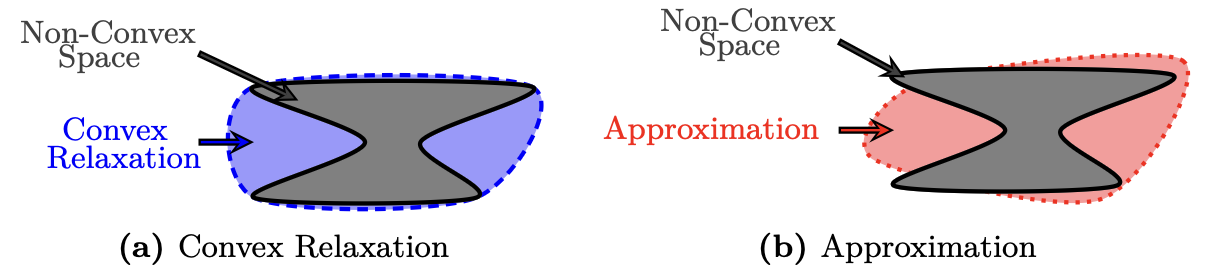
\includegraphics[width=0.9\linewidth]{figuras/relaxacao_aproximacao.png}
}{
\Fonte{adaptado de \citeonline{molzahn2019survey}.}
}
\end{figure}

No painel (a), a relaxação convexa (em azul) \emph{contém} a região não convexa original (em cinza): qualquer ponto factível no problema original continua factível na relaxação, e a relaxação pode incluir pontos adicionais inviáveis. No painel (b), a aproximação (em vermelho) tem um formato distinto da região original, com sobreposição apenas parcial: há pontos factíveis no problema original que ficam fora da aproximação, e há pontos da aproximação que não são factíveis no original. Essa distinção é central para interpretar corretamente os valores de função objetivo discutidos mais adiante: o DC é uma \emph{aproximação} (não fornece limite garantido), enquanto SOC e SDP são \emph{relaxações} (fornecem limite inferior).

As três famílias mais utilizadas na literatura são, conforme \citeonline{molzahn2019survey}:

\begin{alineascomponto}
    \item \textbf{Aproximação DC}: linearização das equações de fluxo sob as hipóteses de tensões próximas a 1\,p.u., ângulos pequenos e perdas desprezíveis. Resulta em um problema de programação linear (LP) de baixíssimo custo computacional, amplamente utilizado em planejamento de longo prazo;
    \item \textbf{Relaxação SOC}: reformulação do FPO em termos de variáveis $W_{ij} = V_i V_j \cos(\theta_i - \theta_j)$ e $T_{ij} = V_i V_j \sin(\theta_i - \theta_j)$, na qual as restrições não convexas são substituídas por desigualdades de cone de segunda ordem. É exata em redes radiais e fornece bons \textit{lower bounds} em redes malhadas;
    \item \textbf{Relaxação SDP}: reformulação como problema de programação semidefinida sobre a matriz $W = V V^H$, mais apertada que a SOC mas computacionalmente mais cara.
\end{alineascomponto}

Embora o presente trabalho não utilize as relaxações DC, SOC ou SDP em sua progressão principal de formulações, que mantém a formulação AC polar não convexa, uma comparação isolada entre as três famílias é apresentada no \textit{script} auxiliar \texttt{CodeComparing.jl}, disponível em \texttt{powerflow/Codes/PowerModels/}, sobre o caso de cinco barras \texttt{case5.m} do \textit{PowerModels.jl}. O objetivo é puramente didático: evidenciar o \textit{gap} existente entre as relaxações e a solução AC exata.

O script resolve o FPO nas três formulações usando o mesmo \textit{solver} (Ipopt) e o mesmo caso de teste, reportando o valor da função objetivo (custo de geração, em US\$/h) em cada caso. Os resultados obtidos foram:

\begin{table}[!htb]
\captionsetup{width=10cm}
\Caption{\label{tab:codecomparing} Comparação de objetivos entre formulações AC, DC e SOC no \texttt{case5.m}}
\IBGEtab{}{
    \begin{tabular}{llr}
        \toprule
        Formulação & Característica & Objetivo (US\$/h) \\
        \midrule \midrule
        AC-OPF & Exata, não convexa & 18\,269{,}10 \\
        DC-OPF & Aproximação linear & 17\,613{,}22 \\
        SOC-OPF & Relaxação convexa & 15\,051{,}45 \\
        \bottomrule
    \end{tabular}
}{
    \Fonte{elaborado pelo autor a partir da execução de \texttt{CodeComparing.jl}.}
}
\end{table}

A leitura da \autoref{tab:codecomparing} ilustra dois comportamentos fundamentais da teoria de relaxações do FPO. Primeiro, o DC-OPF produz um custo \emph{inferior} ao AC-OPF (17\,613 vs.\ 18\,269 US\$/h): como a aproximação linear ignora as perdas ativas e impõe condições de operação irreais (tensões fixas em 1\,p.u.), o problema DC admite despachos que o AC não admite, resultando em um ótimo \emph{infactível} para a rede real que aparece, na escala de custo, abaixo do ótimo verdadeiro. Segundo, o SOC-OPF fornece um custo ainda menor (15\,051 US\$/h), e isso é teoricamente garantido: a relaxação SOC obtida por elevar as variáveis $V_i V_j \cos\theta_{ij}$ e $V_i V_j \sin\theta_{ij}$ a variáveis independentes com restrições de cone de segunda ordem é uma \emph{relaxação} do problema original, o que significa que seu conjunto factível contém o conjunto do AC-OPF. Todo ponto AC-factível é SOC-factível, mas o recíproco não é verdadeiro; logo, o SOC pode atingir custos menores, constituindo uma \textbf{cota inferior provável} para o AC-OPF. O \textit{gap} entre SOC e AC neste caso é de aproximadamente 18\%, o que é típico em redes malhadas onde a condição de patching não é satisfeita.

\section{Ações de controle do programa ANAREDE}
\label{sec:acoes-controle}

As formulações clássicas de FP e FPO descritas nas seções anteriores tratam $V_i$, $\theta_i$, $p^g_k$ e $q^g_k$ como variáveis livres dentro de seus limites caixa. A operação real de um SEP, no entanto, envolve um conjunto de \textbf{ações de controle} que se acoplam a essas variáveis. No programa ANAREDE \cite{chavarry2024}, referência da indústria brasileira, essas ações são tratadas por meio de heurísticas e laços iterativos específicos. Este trabalho considera cinco dessas ações, nomeadas a seguir conforme a sigla utilizada nos arquivos PWF.

\subsection{QLIM: limites de geração reativa}
\label{subsec:qlim}

Em uma barra PV, a tensão $V_i$ é mantida em um \textit{setpoint} $V^{ref}_i$ enquanto o gerador associado é capaz de prover a potência reativa necessária. Quando $q^g_k$ atinge $q^{g,\max}_k$ (ou $q^{g,\min}_k$), a barra é convertida em PQ, $q^g_k$ é fixado no limite e $V_i$ passa a flutuar. Esse comportamento de \textit{type-switching} é central para a operação realista, mas é \emph{descontínuo} e, quando codificado diretamente, conflita com solvers NLP suaves como o Ipopt. Uma forma comum de contorná-lo, adotada neste trabalho, é introduzir uma variável de folga $s^q_l$ no balanço reativo da carga e penalizá-la na função objetivo, mantendo $q^g_k$ dentro dos limites caixa originais.

Na operação real, o QLIM corresponde ao comportamento físico do Regulador Automático de Tensão (RAT) do gerador síncrono. O RAT atua continuamente, em escala de segundos, ajustando a corrente de campo da máquina para sustentar $V^{ref}_i$ nos terminais; sua autoridade de controle, porém, é limitada pela curva de capabilidade do gerador (limites de aquecimento de estator e rotor e limite de estabilidade subexcitado), que define $q^{g,\min}_k$ e $q^{g,\max}_k$. Quando a demanda reativa do sistema empurra $q^g_k$ contra um desses limites, o RAT satura: a corrente de campo trava no valor máximo (ou mínimo) admissível, $q^g_k$ deixa de variar e $V_i$ na barra do gerador passa a depender exclusivamente da rede. Cenários típicos de saturação ocorrem em horários de carga pesada, quando a demanda reativa é alta, e durante contingências (perda de um circuito de transmissão ou de um banco de reativos), em que o sistema exige da geração todo o suporte de tensão disponível. A conversão de PV para PQ que o ANAREDE executa no laço de \textit{type-switching} é, portanto, a representação algébrica desse fenômeno físico.

\subsection{VLIM: limites de magnitude de tensão}
\label{subsec:vlim}

De forma análoga, o controle VLIM trata $V_i$ como variável dentro dos limites caixa $[V^{\min}_i, V^{\max}_i]$, mas adiciona uma restrição de igualdade entre $V_i$ e o \textit{setpoint} $V^{ref}_i$ por meio de uma variável de folga $s^v_i$, também penalizada. Combinado com QLIM, o par de slacks $(s^v_i, s^q_l)$ implementa, na linguagem do otimizador, a mesma lógica que o ANAREDE expressa no laço de \textit{type-switching}.

Na operação real, os limites $[V^{\min}_i, V^{\max}_i]$ correspondem à faixa de tensão na qual cada barra pode operar em regime permanente sem violar normas técnicas e sem comprometer equipamentos conectados. No SIN, esses limites são definidos pelos Procedimentos de Rede do ONS (Submódulo 2.3), que estabelecem faixas de 0,95 a 1,05\,p.u.\ para barras da rede básica em condição normal e tolerâncias mais amplas em emergência. Cargas industriais sensíveis (acionamentos de velocidade variável, fornos a arco) e elementos isolantes (buchas de transformador e para-raios) impõem o limite superior, enquanto o desempenho de motores de indução e a estabilidade de tensão impõem o limite inferior. O \textit{setpoint} $V^{ref}_i$, por sua vez, é o valor programado pela Sala de Controle ou pelo Estudo de Pré-Operação para cada barra controlada: o operador define um perfil de tensão alvo (por exemplo, 1,02\,p.u.\ em barras de 500\,kV em carga leve) e o sistema deve perseguir esse perfil por meio das ações de controle disponíveis. O VLIM é, portanto, a forma algébrica de exigir que a solução do FP respeite simultaneamente os limites normativos e o perfil de tensão programado.

\subsection{CSCA: bancos \textit{shunt} chaveados}
\label{subsec:csca}

Os bancos \textit{shunt} (capacitivos ou indutivos) chaveáveis são representados, no PWF, por uma susceptância $b^{sh}_s$ que pode assumir um conjunto discreto de valores entre $b^{sh,\min}_s$ e $b^{sh,\max}_s$. No ANAREDE, o controle CSCA promove o chaveamento dos passos para manter $V_i$ próxima do \textit{setpoint}. Em uma formulação NLP, $b^{sh}_s$ é tipicamente relaxada para variável contínua dentro do intervalo $[b^{sh,\min}_s, b^{sh,\max}_s]$, representação que será mantida neste trabalho, e a discretização posterior é tratada via \textit{rounding} ou em formulação MINLP.

Na operação real, o CSCA representa o conjunto de bancos de capacitores e reatores manobrados por disjuntor em subestações da rede de transmissão e distribuição. Cada banco é dimensionado em passos discretos, da ordem de dezenas a centenas de MVAr (no SIN, valores típicos vão de 50\,MVAr em subestações de subtransmissão até 200\,MVAr em barras de 500\,kV), e o chaveamento é uma decisão de horizonte mais lento que o RAT: tipicamente, o operador (ou um esquema automático de controle de tensão regional) decide ligar ou desligar um banco com base em medidas de tensão sustentadas por minutos. A motivação típica é o ciclo diário de carga: bancos capacitivos são ligados em horários de carga pesada, quando a tensão tende a cair, e desligados (ou substituídos por reatores) em horários de carga leve, especialmente em sistemas com longas linhas de transmissão pouco carregadas, nas quais o efeito Ferranti eleva a tensão. A relaxação contínua adotada na formulação NLP descarta a granularidade discreta do chaveamento, mas captura corretamente a direção e a magnitude da compensação reativa que o operador realizaria.

\subsection{CTAP: \textit{tap} ajustável de transformadores}
\label{subsec:ctap}

Transformadores em carga (\textit{on-load tap-changer}, OLTC) possuem razão de transformação $t_{ij}$ ajustável, em geral para regulação de tensão na barra do lado de baixa. No PWF, $t_{ij}$ é dada com um valor inicial e limites $[t^{\min}_{ij}, t^{\max}_{ij}]$. O controle CTAP é, novamente, discreto na operação real (passos de 0,5\% a 1\%), mas a relaxação contínua é a representação adotada na formulação NLP utilizada neste trabalho, com uma restrição adicional ligando $V_i$ ao \textit{setpoint} via folga.

Na operação real, o OLTC é um mecanismo eletromecânico que comuta espiras do enrolamento primário (ou terciário) do transformador \emph{sem desenergizar a carga}. A faixa de regulação típica vai de $\pm 10\%$ a $\pm 15\%$ do tap nominal, distribuída em dezesseis a trinta e dois passos. O controlador automático local opera com banda morta (\textit{deadband}) e temporização: ao detectar tensão fora da faixa $V^{ref} \pm \Delta V$ por mais de algumas dezenas de segundos, comanda um passo na direção corretiva. Essa temporização é deliberada e tem dois propósitos: evitar comutações em transitórios curtos (curtos-circuitos, partidas de motores, religamentos) que solicitariam mecanicamente o comutador, e coordenar-se hierarquicamente com o RAT do gerador, que é mais rápido. No SIN, os OLTC equipam transformadores de fronteira entre a rede básica (525 ou 765\,kV) e a rede de subtransmissão (138 ou 230\,kV) e respondem por uma fatia importante do suporte de tensão em regime permanente, complementando os bancos \textit{shunt} (CSCA) e a geração reativa (QLIM). A formulação NLP adotada neste trabalho ignora a temporização e a granularidade dos passos, mas reproduz o efeito em regime permanente: o ajuste de $t_{ij}$ que minimiza o desvio em relação a $V^{ref}$ na barra controlada.

\subsection{DERA: esquema hierárquico de corte/alívio de carga}
\label{subsec:dera}

A sigla DERA é, neste trabalho, o rótulo herdado do nome do \textit{script} \texttt{(F5)+DERA.jl} para designar um esquema de corte hierárquico de carga introduzido sobre a formulação F4. A motivação é que, quando o problema soft-constraint não consegue acomodar todas as exigências de tensão, geração reativa e \textit{setpoints} simultaneamente, um último mecanismo de alívio fica disponível: parte da carga ativa (e da reativa associada, com fator de potência preservado) pode ser cortada nas barras escolhidas pelo solver, com penalidade crescente do nível de tensão mais baixo ao mais alto. Em termos operacionais, esse mecanismo desempenha, dentro da formulação NLP, papel análogo ao do controle de carga em emergência: oferece ao otimizador uma válvula de escape factível quando todas as ações de controle anteriores se esgotam.

Cada carga $l \in \mathcal{L}$ recebe duas variáveis de decisão: $\Delta p^d_l \in [0, p^d_l]$ (corte de potência ativa) e $\Delta q^d_l$ (corte de potência reativa). As duas são acopladas pelo fator de potência nominal da carga por meio da restrição $\Delta q^d_l = \Delta p^d_l \cdot (q^d_l / p^d_l)$, o que evita que o solver corte só ativa ou só reativa de forma desacoplada da característica da carga. Os cortes entram nos balanços nodais subtraindo da demanda nominal:
\begin{equation}
\label{eq:dera-balanco}
p^d_{l,\text{eff}} = p^d_l - \Delta p^d_l, \qquad q^d_{l,\text{eff}} = q^d_l - \Delta q^d_l.
\end{equation}
A função objetivo soft-constraint ganha um termo linear $\sum_{l \in \mathcal{L}} w_l \, \Delta p^d_l$, em que o peso $w_l$ depende do nível de tensão da barra hospedeira da carga. Adotam-se três faixas: $w_l = 10^3$ se $V^{base}_l < 69$\,kV (subtransmissão e distribuição, primeiro recurso de corte), $w_l = 5{\times}10^3$ se $69 \le V^{base}_l \le 230$\,kV (transmissão) e $w_l = 10^4$ se $V^{base}_l > 230$\,kV (extra alta tensão, último recurso). Essa hierarquia inverte a métrica de continuidade do serviço: cortar primeiro nas barras mais ``fáceis de religar'' e preservar ao máximo as cargas servidas em tensão mais alta.

Na operação real, esse tipo de esquema corresponde aos \textbf{Esquemas Regionais de Alívio de Carga (ERAC)} previstos no Submódulo 10.11 dos Procedimentos de Rede do ONS, e a esquemas locais de corte por subfrequência ou subtensão (UFLS/UVLS na literatura internacional). Em campo, esses esquemas são acionados em emergência (perda súbita de geração ou de um corredor de transmissão) e cortam blocos pré-selecionados de carga em escalas de segundos para evitar o colapso. A hierarquia por nível de tensão é uma simplificação operacional do mesmo princípio: cargas em 13,8\,kV (alimentadores de distribuição) costumam ser as primeiras a serem desligadas, enquanto cargas alimentadas diretamente em 230 ou 500\,kV (grandes consumidores industriais, refinarias, indústrias eletrointensivas) são protegidas até onde possível, pois sua reposição é demorada e impacta direto a economia. A formulação NLP adotada substitui o caráter discreto e em emergência do ERAC real por uma decisão contínua de otimização: o solver cortará carga apenas quando isso for mais barato (em termos de função objetivo) do que violar as restrições de tensão das formulações anteriores.

\subsection{Síntese das ações de controle}
\label{subsec:sintese-controles}

As cinco ações descritas nas Seções \ref{subsec:qlim}--\ref{subsec:dera} compõem o conjunto de controles que serão sucessivamente adicionados, no \autoref{chap:metodologia}, sobre uma formulação base de FP em JuMP. A cada controle adicionado, a função objetivo \textit{soft-constraint} ganha um novo termo de penalidade, e o conjunto de variáveis de decisão cresce em $|\mathcal{S}|$ (CSCA), $|\mathcal{B}_{tap}|$ (CTAP) ou $2|\mathcal{L}|$ (DERA), conforme o caso. Esta organização incremental permite isolar, no \autoref{chap:resultados}, o impacto de cada controle sobre a convergência e sobre o ponto de operação calculado.
